\newpage
\hypertarget{rules vis}{}
\subsection{BoxToDictionaryRule}
\genHeader

\begin{enumerate}

\item[$\blacktriangleright$] Select the created subpackage \texttt{src/org.moflon.tgg.mosl.rules} (Step 1 in Fig.~\ref{ea:create_tgg_rule}) and click on the wizard ``Create new TGG rule'' (Step 2).
In the dialogue that pops up, enter \texttt{BoxToDictionaryRule} as the name of the TGG rule to be created.
Open the newly created file.

\begin{figure}[htbp]
\begin{center}
  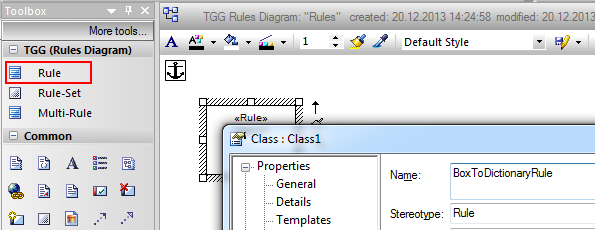
\includegraphics[width=0.8\textwidth]{ea_TGGNewRule}
  \caption{Creating a TGG rule}
  \label{ea:create_tgg_rule}
\end{center}
\end{figure}

\begin{figure}[htbp]
\begin{center}
  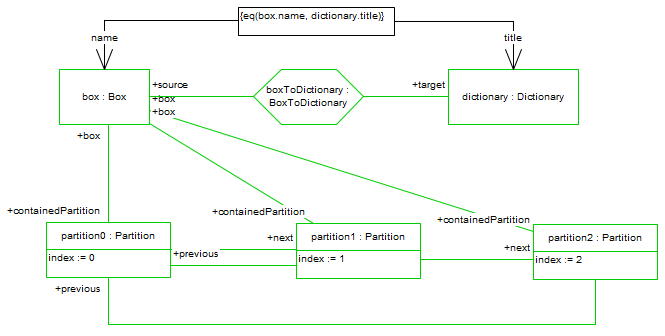
\includegraphics[angle=90,width=\textwidth]{ea_BoxToDictionaryRuleComplete}
  \caption{Complete TGG rule diagram for \texttt{BoxToDictionaryRule}}
  \label{ea:boxtodictionaryrule_complete}
  \end{center}
\end{figure}

\item[$\blacktriangleright$]  Ensure that you open the \texttt{PlantUML} view (Step 1 in Fig.~\ref{ea:boxtodictionaryrule_complete}) as it provides a helpful visualisation of the current TGG rule opened in the editor.
To prevent slowing you down, the view is only updated when you save \emph{and} change your cursor position.
Elements in the source domain have a yellow background, while target elements have a peach background.
Basic UML object diagram syntax is used, extended with colours to represent created elements (green outline) and context elements (black outline).
\texttt{BoxToDictionaryRule} is a so called``island'' rule and only has created elements.
For presentation purposes, correspondence links are abstracted from in the visualisation and are depicted as bands (e.g., between \texttt{box} and \texttt{dictionary}).
The rule we want to specify creates a minimal dictionary (just a \texttt{Dictionary} node), and a minimal box, which is a bit more interesting as it consists already of three correctly connected partitions.
Any structure less than this is not a valid learning box.

\item[$\blacktriangleright$] The textual syntax we use is pretty straightforward:  every domain has a scope (\texttt{\#source}, \texttt{\#target}, and \texttt{\#correspondence}), and there is a final scope for so called attribute conditions, which express how attribute values relate to each other.
The domain scopes contain again scopes for each \emph{object variable} in the rule (e.g., \texttt{box}) and these scopes then contain outgoing \emph{link variables} (e.g., \texttt{-contained\-Partition->}), as well as inline attribute conditions (e.g., \texttt{index := 0}).
Go ahead and specify the source scope as depicted in Step 2 of Fig.~\ref{ea:boxtodictionaryrule_complete}.
Notice how the \texttt{++} operator is used to mark object and link variables as created or context variables.
Try removing and adding it and see how the visualisation changes.  
As always, let the editor help you by pressing ``Ctrl+Space'' as often as possible.

\item[$\blacktriangleright$] Specify the correspondence and target scopes accordingly and make sure your rule (and its visualisation) closely resembles Fig.~\ref{ea:boxtodictionaryrule_complete}.

\item[$\blacktriangleright$] To complete our first rule, specify an attribute condition to declare that the name of the box and the title of the dictionary are always to be equal.
As depicted in Step 3 Fig.~\ref{ea:boxtodictionaryrule_complete}, this can be accomplished using an \texttt{eq} condition.
We provide a standard library of such attribute conditions (press \texttt{F3} on the constraint to jump to the library file), but it is also possible to extend this library with your own attribute conditions.
We'll see how to do this in a moment.
\end{enumerate}

Fantastic work! The first rule of our transformation is complete! 
If you are in hurry, you could jump ahead and proceed directly to Section~\ref{sect:TGGs_in_Action}: TGGs in Action. 
There you can transform a box to a dictionary and vice-versa, but please be aware that your specified TGG (with just one rule) will only be able to cope with completely empty boxes and dictionaries. 
Handling additional elements (i.e., cards in the learning box and entries in the dictionary) requires a second rule.
We intend to specify this next.

\subsection{CardToEntryRule}

Our next goal is to be able to handle \texttt{Card} and \texttt{Entry} elements. 
The new thing here is that it will require a pre-condition -- you should not be able to transform these child elements (cards and entries) unless certain structural conditions (there parents exist and are related) are met. 
In other words, we need a rule that demands an already existing \texttt{box} and \texttt{dictionary}. 
It will need to combine `black' and `green' variables! 

\begin{enumerate}

\item[$\blacktriangleright$] As we'll be connecting cards and entries, we need a new correspondence type.
Open the TGG schema and add a new correspondence type \texttt{CardToEntry} connecting a \texttt{Card} and an \texttt{Entry}.

\item[$\blacktriangleright$] Create a new TGG rule with \texttt{Card\-To\-Ent\-ry\-Rule} its name, and specify the rule as depicted in Fig.~\ref{ea:cardtoentry_1}.
\end{enumerate}

Your diagram should now resemble Fig.~\ref{ea:cardtoentry_1}. 
We're not done yet though, we still need to handle attributes!
To understand why, consider the current rule and ask yourself  \emph{which} partition is meant.
Exactly!  This is currently not specified, so \emph{any} partition can be taken when applying the rule.
eMoflon would actually collect all applicable rules (one for every partition) and consult a configuration component to decide which rules should be taken.
The default component just chooses randomly, but you could override this and e.g., pop up a dialogue asking the user which partition is preferred.
Although this could be an interesting solution, we'll see how to fully specify things using extra attribute conditions.

\begin{figure}[htbp]
  \begin{center}
    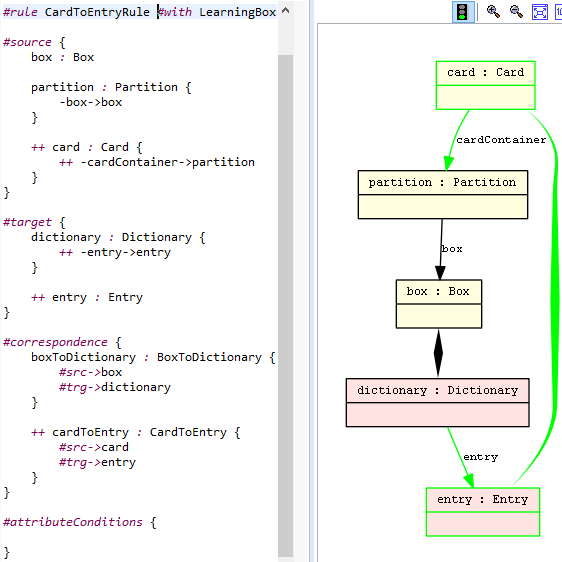
\includegraphics[width=\textwidth]{ea_cardToEntryRule}
    \caption{\texttt{CardToEntryRule} without attribute manipulation}
    \label{ea:cardtoentry_1}
  \end{center}
\end{figure}

On the way to handling all attributes, let's first start with the relatively easy case of specifying how every \texttt{entry\-.cont\-ent}, \texttt{card.back}, and \texttt{card.face} relate to each other.
We should probably combine the front and back of each card as a single content attribute of an entry and, in the opposite direction, split the content into \texttt{card.back} and \texttt{card.face}.

So let's define \texttt{entry\-.cont\-ent} as: \texttt{<word>:<mean\-ing>}. 
\texttt{card\-.back} should therefore be \texttt{Quest\-ion:<word>} and similarly, \texttt{card\-.face} should be \texttt{Ans\-wer:<mean\-ing>}. 

\begin{enumerate}
\item[$\blacktriangleright$] Luckily, we have two library attribute conditions, \texttt{addPrefix} and \texttt{concat} to help us with this.
Add the following to your rule:

\verb|addPrefix("Question", word, card.back)|\\  
\verb|addPrefix("Answer", meaning, card.face)|\\
\verb|concat(":", word, meaning, entry.content)|

``Question'' and ``Answer'' are EString literals, \texttt{word} and \texttt{meaning} are local variables, and \texttt{card.face}, \texttt{card.back}, and \texttt{entry.content} are attribute expressions (this should be familiar from SDM story patterns).

\item[$\blacktriangleright$] Our final task is now to specify where a new \texttt{card} (when transformed from an \texttt{entry}) should be placed.  
We purposefully created three partitions to match the three difficulty levels, but if you check the available library constraints, there is nothing that can directly implement this specific kind of mapping. 
We will therefore need to create our own attribute condition to handle this.

\item[$\blacktriangleright$] Open the TGG schema, and define a new attribute condition in the \texttt{\#attributeConditions} scope. 
Name it \texttt{IndexToLevel}, and enter the values given in Fig. \ref{ea:create_new_constraint}.

\begin{figure}[htbp]
\begin{center}
  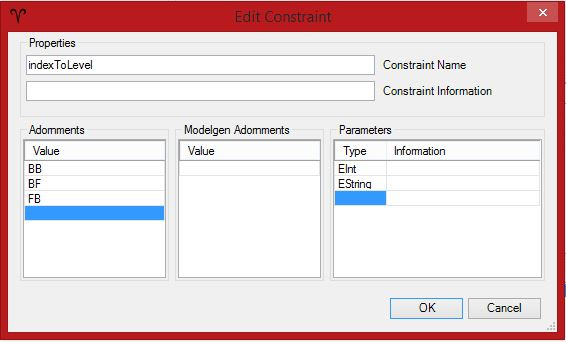
\includegraphics[width=0.55\textwidth]{ea_uniqueConstraint}
  \caption{Specifying a new attribute condition}
  \label{ea:create_new_constraint}
\end{center}
\end{figure}
\FloatBarrier

\item[$\blacktriangleright$] Please note that this is just a \emph{specification} of a custom attribute condition -- we still need to actually implement it in Java! 
As we're so close to finishing this TGG rule, however, let's complete it first before we work out the exact meaning of the mysterious adornments (those funny \texttt{BB}, \texttt{BF}, \dots) and parameters (\texttt{0:EInt} and \texttt{1:EString}) of the attribute condition. 
For now, just make sure you enter the exact values in Fig.~\ref{ea:create_new_constraint}. 

\item[$\blacktriangleright$] We can now use this new attribute condition just like any of the library attribute conditions.
Add the following to \texttt{CardToEntryRule} to express that the relationship between the index of the partition containing the new card, and the level of the new entry, is defined by our new attribute condition:

\verb|indexToLevel(partition.index, entry.level)|
\end{enumerate}

Great work! All that's left to do is implement the \texttt{indexToLevel} constraint, and give your transformation a test run.


%%% Local Variables: 
%%% mode: latex
%%% TeX-master: "../src/TGG_mainFile"
%%% End: 
